\documentclass[12pt, a4paper]{report}
\usepackage{epsfig}
\usepackage{subfigure}
%\usepackage{amscd}
\usepackage{amssymb}
\usepackage{graphics}
\usepackage{graphicx}
%\usepackage{amscd}
\usepackage{amssymb}
\usepackage{subfiles}
\usepackage{framed}
\usepackage{subfiles}
\usepackage{amsthm, amsmath}
\usepackage{amsbsy}
\usepackage{framed}
\usepackage[usenames]{color}
\usepackage{listings}
\lstset{% general command to set parameter(s)
	basicstyle=\small, % print whole listing small
	keywordstyle=\color{red}\itshape,
	% underlined bold black keywords
	commentstyle=\color{blue}, % white comments
	stringstyle=\ttfamily, % typewriter type for strings
	showstringspaces=false,
	numbers=left, numberstyle=\tiny, stepnumber=1, numbersep=5pt, %
	frame=shadowbox,
	rulesepcolor=\color{black},
	,columns=fullflexible
} %
%\usepackage[dvips]{graphicx}
\usepackage{natbib}
\usepackage{epstopdf}
\bibliographystyle{chicago}
\usepackage{vmargin}
% left top textwidth textheight headheight
% headsep footheight footskip
\setmargins{3.0cm}{2.5cm}{15.5 cm}{22cm}{0.5cm}{0cm}{1cm}{1cm}
\renewcommand{\baselinestretch}{1.5}
\pagenumbering{arabic}
\theoremstyle{plain}
\newtheorem{theorem}{Theorem}[section]
\newtheorem{corollary}[theorem]{Corollary}
\newtheorem{ill}[theorem]{Example}
\newtheorem{lemma}[theorem]{Lemma}
\newtheorem{proposition}[theorem]{Proposition}
\newtheorem{conjecture}[theorem]{Conjecture}
\newtheorem{axiom}{Axiom}
\theoremstyle{definition}
\newtheorem{definition}{Definition}[section]
\newtheorem{notation}{Notation}
\theoremstyle{remark}
\newtheorem{remark}{Remark}[section]
\newtheorem{example}{Example}[section]
\renewcommand{\thenotation}{}
\renewcommand{\thetable}{\thesection.\arabic{table}}
%\renewcommand{\thefigure}{\thesection.\arabic{figure}}
\title{Research notes: linear mixed effects models}
\author{ } \date{ }


\begin{document}
	\author{Kevin O'Brien}
	\title{Mixed Models for Method Comparison Studies}
	\tableofcontents
	
	%----------------------------------------------------------------------------------------%
	\newpage
	
%-- Paragraph 1a
\chapter{Established Techniques for Method Comparison Studies}
\section{Techniques for Simple Design Studies}
The issue of whether two methods of measurements are 
comparable to the extent that they can be used 
interchangeably with sufficient accuracy and measurement precision is encountered frequency in scientfic research. Published examples of method comparison studies can be found in disciplines
as diverse as pharmacology \citep{ludbrook97}, anaesthesia \citep{Myles}, and cardiac imaging methods \citep{Krumm}(references).

%-- Paragraph 1B
%-- Paragraph 1C

In the most basic design, items (i.e. people in medical studies) are measures once only by each of two measurement methods. 
If the recorded measurements by the two instruments differ systematically, a problem of inter-method bias exists. Oftentimes this bias can be mitigated by some technical adjustment or recalibration of the readings. However, if the method variances differ, no comparable adjustment is possible, and a more serious problem exists.



%-- Paragraph 1D

This problem has received significant attention in statistical literature over many decades.
Statistical tests for equality of measurements precisions were devised by \citet{pitman} and \citet{morgan}. \citet{Grubbs48,Grubbs73} formulate a model testing framework for comparing multiple devices.



%-- Paragraph 2A
%-- Paragraph 2B

A graphical tool advocated by \citet{BA83,BA86} shifted the analysis from concerns over statistical hypothesis testing to concerns of statistical equivalence. Known as the Bland-Altman plot, this technique has become the most popular (and in some cases, obligatory) method of presenting method comparison studies in journals. \citet{DunnSEME} prefers an approach based in measurement error models. \citet{BXC2008} extend the technique to replicated deisign using LME frameworks to replicated designs using an LME framework, and supports this work with an \texttt{R} package. \citet{broemeling2009} lays out a Bayesian strategy.


With some few exceptions, e.g. \citet{hawkins1978} and \citet{Bartko}, the issue of outliers and anomalous values have not featured prominently in method comparison literature, a topic that we will particular attention to in a later chapter.

%-- Paragraph 2C

This chapter is organized as follows; firstly a review of the tools used in the analysis of unreplicated deisgns. We then consder ther extension to replicated designs. The LME framework advanced by \citet{BXC2008} and \citet{ARoy2009} are given special attention.


%-- Paragraph 3A



\section{Conventional Approaches to Unreplicated Design}  
Let the random variables $Y_1$ and $Y_2$ be distributed bivariate normal with $\mathrm{E}(Y_1)=\mu_1,\ \mathrm{E}(Y_2)=\mu_2,\ \mathrm{var}(Y_1)=\sigma^2_1,\ \mathrm{var}(Y_2)=\sigma^2_2,$ and correlation coefficient $-1<\rho<1.$ Of particular interest are tests of the unconditional marginal hypotheses $\textrm{H}^\prime\colon~\mu_1 = \mu_2$ and $\textrm{H}^{\prime\prime}\colon~\sigma^2_1 = \sigma^2_2,$ and tests of the joint hypothesis $\textrm{H}^\mathrm{J}\colon~\mu_1 = \mu_2\ \textrm{and}\ \sigma^2_1 = \sigma^2_2.$ The random variables $D=Y_1-Y_2$ and $S=Y_1+Y_2$ are bivariate normal with expectations $\mathrm{E}(D) = \mu_D = \mu_1- \mu_2$ and $\mathrm{E}(S) = \mu_S = \mu_1+ \mu_2,$ variances $\mathrm{var}(D) = \sigma^2_D = \sigma_1^2 + \sigma_2^2 - 2 \rho \sigma_1 \sigma_2$ and $\mathrm{var}(S) = \sigma^2_S = \sigma_1^2 + \sigma_2^2 + 2 \rho \sigma_1 \sigma_2,$ and covariance $\mathrm{cov}(D,S) = \sigma_1^2 - \sigma_2^2.$ The conditional distribution of $D$ given $S$ is normal with expectation $\mu_{D\mid S=s} = \mu_D + [ ( \sigma^2_1 - \sigma^2_2 ) / \sigma^2_S ] ( s - \mu_S )$ and variance $\sigma^2_{D\mid S} = \sigma^2_D - ( \sigma^2_1 - \sigma^2_2 )^2 / \sigma^2_S.$ These differences and sums are the building blocks of the test procedures: of $\textrm{H}^\prime,$ due to \cite{Student}; of $\textrm{H}^{\prime\prime}$, devised concurrently by \cite{pitman} and \cite{morgan}; and of $\textrm{H}^\mathrm{J},$ proposed by \citet{BB89}. Notably, the classic test procedure of $\textrm{H}^\prime$ due to \cite{Student} makes no assumptions about the equality, or otherwise, of the variance parameters $\sigma^2_1$ and $\sigma^2_2.$

The test procedure for $\textrm{H}^\mathrm{J}$ advanced by \citet{BB89} additively decomposes into independent tests of $\textrm{H}^{\prime\prime}$ and the conditional marginal hypothesis $\textrm{H}^\dag\colon~\mu_1 = \mu_2,$ assuming the additional restriction $\sigma^2_1 = \sigma^2_2.$  The former test in this decomposition is the Pitman-Morgan procedure referred to above. The latter test in the decomposition is based on the $F$-ratio with $(1,n-2)$ degrees-of-freedom, denoted below by $F_0^\ast.$ Conveniently, all three test procedures can be calculated from the fitted simple linear regression of observed differences on observed sums. 



\subsection{The Pitman-Morgan test}

The test of the hypothesis that the variances $\sigma^2_1$ and $\sigma^2_2$ are equal, which was devised concurrently by \cite{pitman} and \cite{morgan}, is based on the correlation of $D$ with $S,$ the coefficient being $\rho_{DS} = (\sigma^2_1 - \sigma^2_2) / (\sigma_D \sigma_S ),$ which is zero if, and only if, $\sigma^2_1 = \sigma^2_2.$ Consequently a test of $\textrm{H}^{\prime\prime}\colon\ \sigma^2_1 = \sigma^2_2$ is equivalent to a test of $\textrm{H}\colon\ \rho_{DS}=0$ and the test statistic is the familiar {\it t}-test for a correlation coefficient with $(n-2)$ degrees-of-freedom:  
\[
T^*_\mathrm{PM} = R \sqrt{ \frac{n-2}{1-R^2} },
\]
where $R =  \sum (D_i-\bar{D})(S_i-\bar{S}) / [ \sum(D_i-\bar{D})^2 \sum (S_i-\bar{S})^2 ]^{\frac{1}{2}} $ 
is the sample correlation coefficient of the $n$ case-wise differences $D_i = Y_{i1} - Y_{i2}$ and sums $S_i = Y_{i1} + Y_{i2}.$ Throughout this paper the summation $\sum$ is taken to imply $\sum_{i=1}^n.$  The procedure is to reject the hypothesis $\textrm{H}^{\prime\prime}$ in favour of $\sigma^2_1\neq\sigma^2_2$ if $|T^*_\mathrm{PM}| >  t_{\alpha/2,(n-2)\textrm{df}}.$ 




\section*{Bland-Altman Plots}

\citet{BA83} correctly criticised the use the paired differnce reegresion and correlation anlayss for use in method comparison. Their graphical procedure is based on pair-wise differences versus pair-wise averages. This plot is essentially a visual analogue of the quantities underpinning the tests presented previously.


%===================================================================================================================%

%-- Paragraph 4A
The plot of differences versus average can be obtained by rotating the points in the original scatterplot of X and Y by 45 degrees and rescaling accordingly. This plot, in essence, serves the purpose of a diagnostic plot.
From a historical perspective, a similar graphical tool was devised by Tukey several decades earlier \citet{kozak2014including}.

%-- Paragraph 4B
We will illustrate the workings of a Bland-Altman plot through a simple example. The data contain in the table below was presented in \citep{Grubbs48}. In each of twelve experimental trials, a single round of ammunition was fired from a 155mm artillery piece and its velocity was measured simultaneously (and independently) by three chronographs devices, identified here by the labels `Fotobalk', `Counter' and `Terma'.
\begin{table}[h!]
	\renewcommand\arraystretch{0.7}%
	\begin{center}
		\begin{tabular}{|c||c|c|c||c|c|c|c|}
			\hline
			Round & Fotobalk  & Counter & Terma  &   &    &   &   \\
			&  [F] & [C] & [T] &[F-C] &  [(F+C)/2] & [F-T] &  [(F+T)/2] \\
			\hline
			1 & 793.8 & 794.6 & 793.2 & -0.8 & 794.2 & 0.6 & 793.5 \\
			2 & 793.1 & 793.9 & 793.3 & -0.8 & 793.5 & -0.2 & 793.2 \\
			3 & 792.4 & 793.2 & 792.6 & -0.8 & 792.8 & -0.2 & 792.5 \\
			4 & 794.0 & 794.0 & 793.8 & 0.0 & 794.0 & 0.2 & 793.9 \\
			5 & 791.4 & 792.2 & 791.6 & -0.8 & 791.8 & -0.2 & 791.5 \\
			6 & 792.4 & 793.1 & 791.6 & -0.7 & 792.8 & 0.8 & 792.0 \\
			7 & 791.7 & 792.4 & 791.6 & -0.7 & 792.0 & 0.1 & 791.6 \\
			8 & 792.3 & 792.8 & 792.4 & -0.5 & 792.5 & -0.1 & 792.3 \\
			9 & 789.6 & 790.2 & 788.5 & -0.6 & 789.9 & 1.1 & 789.0 \\
			10 & 794.4 & 795.0 & 794.7 & -0.6 & 794.7 & -0.3 & 794.5 \\
			11 & 790.9 & 791.6 & 791.3 & -0.7 & 791.2 & -0.4 & 791.1 \\
			12 & 793.5 & 793.8 & 793.5 & -0.3 & 793.6 & 0.0 & 793.5 \\
			\hline
		\end{tabular}
		\caption{Fotobalk : Differences and Averages with counter and terma.}
		\label{GrubbsData1}
	\end{center}
\end{table}
The Bland-Altman plot for comparing the `Fotobalk' and `Counter' methods, which shall henceforth be referred to as the `F vs C' comparison, is depicted on the right in Figure~\ref{fig:FotobalkVsCounter}. The dashed line in the Bland-Altman plot alludes to the inter-method bias between the two methods, estimated by calculating the average of the differences. In the case of Grubbs data the inter-method bias is $-0.61$ metres per second. By inspection of the plot, one would notice that the differences tend to increase as the averages increase.
%\begin{figure}
%\centering
%\includegraphics[width=0.7\linewidth]{images/GrubbsBAplot-LOA}
%\caption{Bland-Altman plot for Artillery Round Data \citet{Grubb48}}
%\label{fig:GrubbsBAplot-LOA}
%\end{figure}

\begin{figure}
\centering
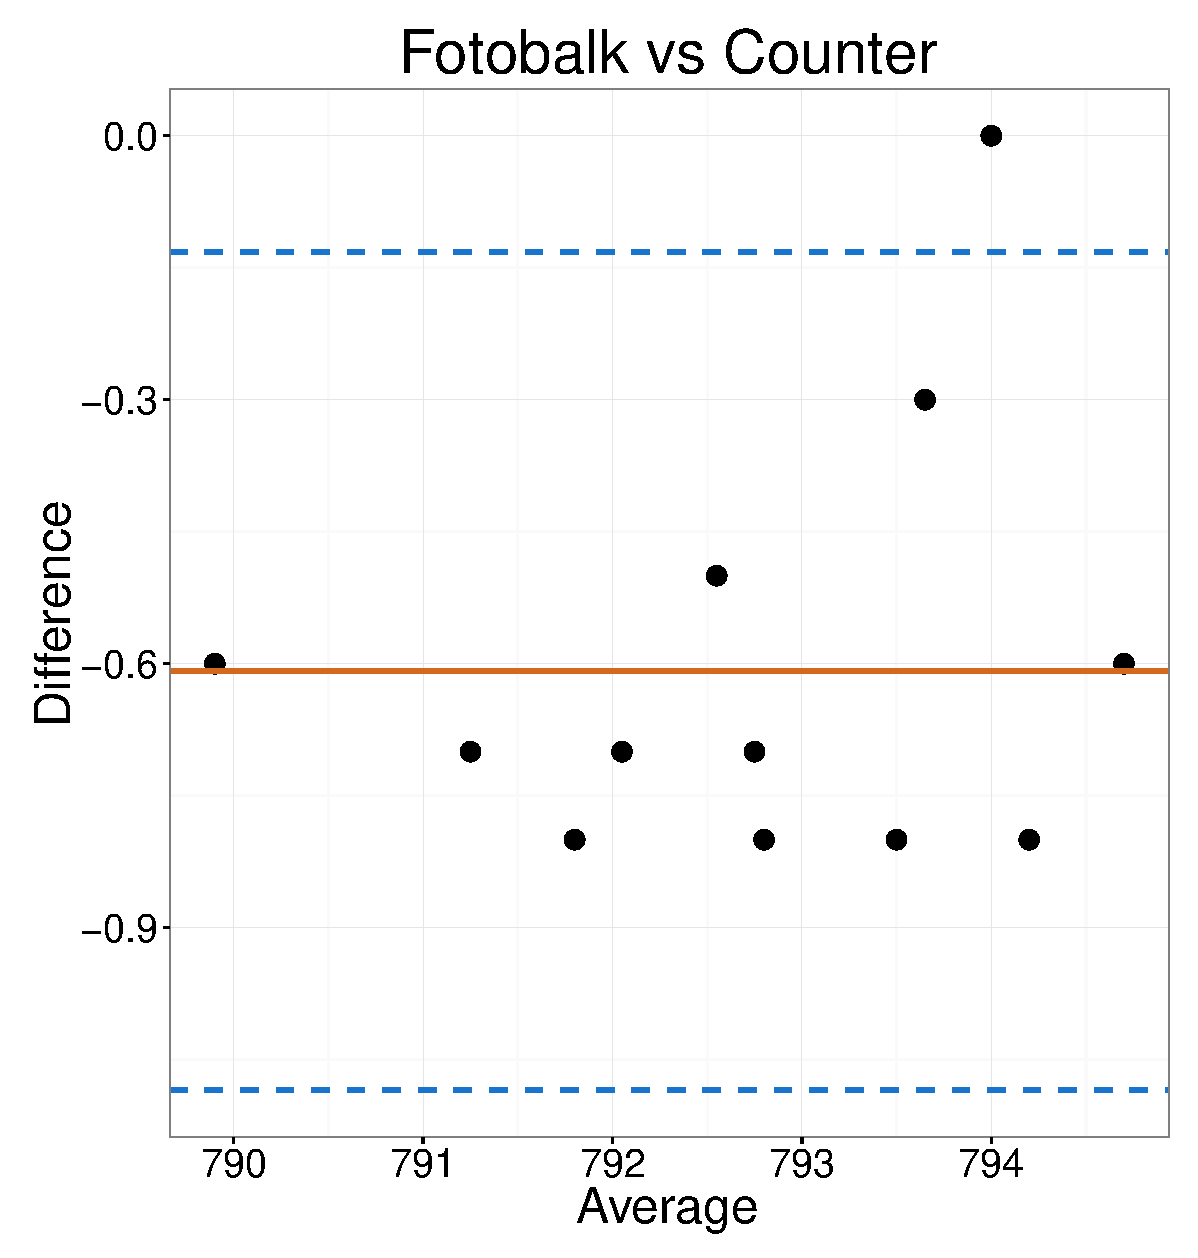
\includegraphics[width=0.55\linewidth]{images/FotobalkVsCounter}
\caption{}
\label{fig:FotobalkVsCounter}
\end{figure}




The values in the final two columns contain the pairwise differences $d_i = x_i - y_i$ and $a_i = {(x_i + y_i)/2} $.

%-- Paragraph 4C
%-- Paragraph 4D

A plot of this quantities is show in figure 1. Also included is a horizontal grey line repesenting th mean of the differences $\bar{d}$. The horizontal dotted lines refer to the limits of agreement and are placed two standard deviations above and below $bar{d}$. The rationale for this plot is that methods showing good agreement would be expected to  have values falling predominantly between the limits of agreement.

%===================================================================================================================%

%-- Paragraph 5A
%-- Paragraph 5B
\citet{BA86} suggested that exact LOAs can be obtained by placing 1.96 in place of the 2 as a multiplier. \citet{BA99} revised this multiplier to be a $t$ value with $n-1$ degrees of freedom for the appropriate coverage.
\citet{BXC2008} argued that prediction intervals are the appropriate tool for deciding the placment of limits of agreement, and these can be calculated as

\[ \bar{d} \pm t_{n-1}.\left[ \sqrt{S.E(\bar{d})} \times \frac{n-1}{\sqrt{1 + (1/n)}} \right]. \]

%-- Paragraph 5C

\citet{BA83} supplement their graphical tool wth a test of the equality of variances, based on the Pitman-Morgan procedure. This test was omitted from their Lancet paper \citep{BA86}, but was mentioned again in \citet{BA99}. In \citet{BA99}, they argue that they don't see a role in hypothesis testing in establishing equivalence of measurement methods.
% Does it re-appear.


%-- Paragraph 5D
%-- DONE



%=============================================================================%
%Paragraph 6
%Much of this analysis is based on classical assumptions of normally distributed data.

Enhancements proposed by \citet{BA99}, such as the use of confidence interval estimates for limits of agreement, have been seldom used in practice.

\section{Generalized Model Designs}
Thus far, the approaches discussed have been based on a simple design, whereby an item is measured by two measurement methods. For method comparison problems, two levels of sophistication exist beyond the simple design. 

The first generalization of the design accounts for comparing two instruments when replicate measurements are present. \citet{ARoy2009} considers two instruments with replicate measurements a developing a testing framework based on linear mixed effects models.

The second generalization accounts of multiple methods of measurement, e.g. the framework proposed by \citet{Grubbs73}. \citet{BXC2008} extends the Bland-Altman framework, also using LME models, to allow for pair-wise comparison of instruments between multiple methods of measurement. \citet{christensenblackwood} present a multivariate linear model for method comparison based on Grubbs's model. Their approach generates the multiple  correlation test for equality of device variances, and yields a new simultaneous test for equality of variances and biases.


The original Bland-Altman method was developed for two sets of measurements done on one occasion, and so this approach is not suitable for replicate measures data, other than a preliminary exploration of the data. \citet{BA99} addresses the issue of computing LOAs in the presence of replicate measurements, suggesting several computationally simple approaches. When repeated measures data are available, it is desirable to use all the data to compare the two methods. 




\section{Prevalence of the Bland-Altman Plot}

\citet*{BA86}, which further develops the Bland-Altman approach,
was found to be the sixth most cited paper of all time by \citet{BAcite}. \cite{Dewitte} reviews the use of Bland-Altman plots by examining all articles in the journal `Clinical Chemistry' between 1995 and 2001, describing the rate at which
prevalence of the Bland-Altman plot has developed in scientific
literature. This study concludes that use of the Bland-Altman plot increased over the years, from 8\% in 1995 to
14\% in 1996, and 31-36\% in 2002.

The Bland-Altman plot has since become the expected, and often the obligatory, approach for presenting method comparison
studies in many scientific journals \citep{hollis}. Furthermore \citet{BritHypSoc} recommend its use in papers pertaining to
method comparison studies for the journal of the British Hypertension Society.


% %	\section{Bland Altman Plots In Literature}
\citet{mantha} contains a study on the use of Bland Altman plots of 44 articles in several named journals over a two year period. 42 articles used Bland Altman's limits of agreement, while the other two used correlation and regression analyses. \citet{mantha} remark that 3 papers, from 42 mention predefined maximum width for limits of agreement that would not impair medical care.

The conclusion of \citet{mantha} is that there are several inadequacies and inconsistencies in the reporting of results, and
that more standardization in the use of Bland-Altman plots is required. The authors recommend the prior determination of limits of agreement before the study is carried out. This contention is endorsed by \citet{lin}, which makes a similar recommendation for the sample size, noting that\emph{``sample sizes required either was not mentioned or no rationale for its choice was given"}.

\begin{quote}
	\textit{In order to avoid the appearance of ``data dredging", both the
		sample size and the (limits of agreement) should be specified and
		justified before the actual conduct of the trial.} \citep{lin}
\end{quote}

\citet{Dewitte} remark that the limits of agreement should be
compared to a clinically acceptable difference in measurements.

\section{Criticism of Limits of Agreement}
The Bland-Altman approach is well noted for its ease of use, and can be easily implemented with most software packages. Also it does not require the practitioner to have more than basic statistical training. The plot is quite informative about the variability of the differences over the range of measurements. For
example, an inspection of the plot will indicate the `fan effect' or the presence of an outlier.





%
%
%How this relates the overall population is unclear. It seems that
%it depends on an expert to decide whether or not the range of
%differences is acceptable. In a study A Bland-Altman plots compare
%two assay methods. It plots the difference between the two
%measurements on the Y axis, and the average of the two
%measurements on the X axis

However the approach comes in for criticism in a number of respects. In the first instance, some caution must be given to the inter-method bias estimate.
If one method is sometimes higher, or sometimes lower, the average of the differences will be close to zero. If the inter-method bias is close to zero, there be an indication that the two measurement methods are in agreement, when in fact they are producing different results systematically.

Several problems have been highlighted regarding limits of agreement. One is the somewhat arbitrary manner in which they are constructed. Limits of agreement are intended to analyse equivalence. How this is assessed is the considered judgement of the practitioner. In \citet{BA86} an example of good agreement is cited. For two methods of measuring `oxygen saturation', the limits of agreement are calculated as (-2.0,2.8) percentage points. According to the authors, a knowledgeable practitioner in the field should ostensibly find this to be sufficiently narrow. If the limits of agreement are not clinically important, which is to say that the differences tend not to be substantial, the two methods may be used interchangeably. Furthermore \citet{DunnSEME} takes issue
with the notion of `equivalence', remarking that while agreement
indicated equivalence, equivalence does not reflect agreement.


While in essence they are similar to confidence intervals, limits of agreement are not constructed as such; they are designed for future values. Lack of clarity in this regards can give rise to confusion, and incorrect interpretations.

\citet{ludbrook97,ludbrook02} criticizes Bland-Altman plots on the basis that they present no information on effect of constant bias or proportional bias. These plots are only practicable when both methods measure in the same units, hence they are totally
unsuitable for conversion problems. There is no guidance on how to deal with outliers. Bland and Altman recognize the effect they would have on the limits of agreement, but offer no guidance on how to correct for those effects. Finally the adaptation of the approach to deal with replicate measurements, as specified by \citet{BA99}, is flawed.
%=====================================================================================================================%
% Paragraph 7A

%- Roy and Carstensen

\section{LME Models in Method Comparison Studies}
When repeated measures data are available for the the computation of the limits of agreement, it is desirable to use all the data to compare the two methods. The classical Bland-Altman method was developed for two sets of measurements done on one occasion, but is inadequate for replicate measurement data. 

\citet{BA99} addressed this issue by suggesting several computationally simple approaches.  One approach suggested by \citet{BA99} is to calculate the mean for each method on each subject and use these pairs of means to compare the two methods. Their second approach is to treat each measurement separately. 
	
The estimate of bias will be unaffected using this approach, but the estimate of the standard deviation of the differences will be too small, because of the reduction of the effect of repeated measurement error \citep{BXC2004,BXC2008}. These authors recommends that replicate measurements be used for each method, but recognizes that resulting data are more difficult to analyze. To this end, they recommend the use of LME models as a suitable framework.
	%\citet{ARoy2009} uses an LME model approach to provide a set of formal tests for method comparison studies.
	
	%\citet{BXC2008} demonstrate statistical flaws with two approaches proposed by \citet{BA99} for the purpose of calculating the variance of the inter-method bias when replicate measurements are available.	
	
	%\citet{BXC2008} demonstrated how the limits of agreement calculated solely from the mean of replicates are `much too narrow as
	%prediction limits for differences between future single measurements'. Carstensen attends to this issue also, adding that another approach would be to treat each repeated measurement separately. 
	
	%This paper also comments that, while treating the
	%replicate measurements as independent will cause a downward bias on the limits of agreement calculation, this method is preferable to the `mean of replicates' approach. 
	
	
	\citet{BXC2008} extends the well established Bland-Altman methodology for the case of replicate measurements on each item by using LME models, to allow for a more statistically rigourous approach to computing appropriate estimates for the variance of the inter-method bias. As their interest mainly lies in extending the Bland-Altman approach, other formal tests are not considered.  
	
	%Measures of repeatability, a
	%characteristic of individual methods of measurements, are also
	%derived using this method.
	
	
	
	
	\subsection{Test For Inter-Method Bias in the LME Frameworks}
	The presence of an inter-method bias is the source of disagreement between two methods of measurement that is most easily identified. A formal test for this can be implemented by examining the fixed effects of the LME model, which model the inter-method bias. This is common to classical linear model, and interpretation of the results should pose not difficulty to a trained practitioner.
	
	The null hypotheses $H_1$, that both methods have the same mean, which is tested against the alternative hypothesis $K_1$ , that both methods have different means;
	\begin{eqnarray}
	\operatorname{H_1} : \mu_1 = \mu_2 ,\\
	\operatorname{K_1} : \mu_1 \neq \mu_2.
	\end{eqnarray}
	The inter-method bias and necessary test statistic and $p-$value are presented in computer output. 
	%================================================================%
	
	\subsection{Limits of Agreement in LME models}
%	
%	Carstensen's approach is that of a standard two-way mixed effects ANOVA with replicate measurements. With regards to the specification of the variance terms, Carstensen remarks that using his approach is common, remarking that ``The only slightly non-standard feature is the differing residual variances between methods" \citep{BXC2010}.
	
	%Carstensen specifies the variance of the interaction terms as being univariate normally distributed. As such, $\mathrm{Cov}(c_{mi}, c_{m^\prime i})= 0.$
\citet{BXC2008} recommend a fitted LME model to obtain appropriate estimates for the variance of the inter-method bias. Their interest lies in generalizing the limits-of-agreement (LOA) method developed by \citet{BA86} to take proper cognizance of the replicate measurements.  Estimation of repeatability is included in this framework, but other formal tests are not considered. The model is constructed to describe the relationship between a value of measurement and its real value. The non-replicate case is considered first, as it is the context of the Bland-Altman plots. This model assumes that inter-method bias is the only difference between the two methods.		

%A measurement $y_{mi}$ by method $m$ on individual $i$ is formulated as follows;
%	\begin{equation}
%	y_{mi}  = \alpha_{m} + \mu_{i} + e_{mi} \qquad ( e_{mi} \sim
%	N(0,\sigma^{2}_{m}))
%	\end{equation}
	
	The following model (in the authors own notation) is
	formulated as follows, where $y_{mir}$ is the $r$th replicate
	measurement on subject $i$ with method $m$. The differences are expressed as $d_{i} = y_{1i} - y_{2i}$.
	\begin{equation}
	y_{mir}  = \alpha_{m} + \beta_{m}\mu_{i} + c_{mi} + e_{mir} \qquad
	( e_{mi} \sim N(0,\sigma^{2}_{m}), c_{mi} \sim N(0,\tau^{2}_{m}))
	\end{equation}
	The intercept term $\alpha$ and the $\beta_{m}\mu_{i}$ term follow from \citet{DunnSEME}, expressing constant and proportional bias
	respectively, in the presence of a real value $\mu_{i}$. $c_{mi}$ is a interaction term to account for replicate, and $e_{mir}$ is the residual associated with each observation. Since variances are specific to each method, this model can be
	fitted separately for each method.
	
This formulation doesn't require the data set to be balanced, but does require a sufficient number of replicates and measurements to overcome the problem of identifiability. Consequently more than two methods of measurement may
be required to carry out the analysis. There is also the assumptions that observations of measurements by particular methods are exchangeable within subjects. The quality of exchangeability means that future samples from a population behaves like earlier samples. For the replicate case, an interaction term $c$ is added to the model, with an associated variance component. All the random effects are assumed independent, and that all replicate measurements are assumed to be exchangeable within each method. 
	
%%	\citet{BXC2008} presents a simplified, but more tractable, model:
%%	\begin{equation}
%%	y_{mir}  = \alpha_{m} + \mu_{i} + c_{mi} + e_{mir} \qquad ( e_{mi}
%%	\sim N(0,\sigma^{2}_{m}), c_{mi} \sim N(0,\tau^{2}_{m}))
%%	\end{equation}
%%	Modern software packages can be used to fit models accordingly. The best linear unbiased predictor (BLUP) for a specific subject $i$ measured with method $m$ has the form $BLUP_{mir} = \hat{\alpha_{m}} +
%%	\hat{\beta_{m}}\mu_{i} + c_{mi}$, under the assumption that the
%%	$\mu$s are the true item values.
%%	
	
	
	%\citet{BXC2004} uses the above formula to predict observations for
	%a specific individual $i$ by method $m$;
	%
	%\begin{equation}BLUP_{mir} = \hat{\alpha_{m}} + \hat{\beta_{m}}\mu_{i} +
	%c_{mi}. \end{equation} Under the assumption that the $\mu$s are
	%the true item values, this would be sufficient to estimate
	%parameters. When that assumption doesn't hold, regression
	%techniques (known as updating techniques) can be used additionally
	%to determine the estimates. 
	%
	%The assumption of exchangeability can
	%be unrealistic in certain situations. \citet{BXC2004} provides an
	%amended formulation which includes an extra interaction term=, $
	%d_{mr} \sim N(0,\omega^{2}_{m}$, to account for this.
	
	%\citet{BXC2004} uses the above formula to predict observations for
	%a specific individual $i$ by method $m$;
	
	
%	
%	\subsection{Carstensen's LME Framework for Method Comparison}
	
	
	
%	%These authors advocate a LME model for the purpose of comparing two methods of measurement where replicate measurements are available on each item. 
%	%
%
%	
%	A measurement $y_{mi}$ by method $m$ on individual $i$ is
%	formulated as follows;
%	
%	\begin{equation}
%	y_{mi}  = \alpha_{m} + \mu_{i} + e_{mi} \qquad ( e_{mi} \sim
%	N(0,\sigma^{2}_{m}))
%	\end{equation}
%	
%
%	
%	\citet{BXC2004} presents a model to describe the relationship between a value of measurement and its real value. The non-replicate case is considered first, as it is the context of the Bland Altman plots. This model assumes that inter-method bias is the only difference between the two methods. A measurement $y_{mi}$ by method $m$ on individual $i$ is formulated as follows:
%	\begin{equation}
%	y_{mi}  = \alpha_{m} + \mu_{i} + e_{mi} \qquad ( e_{mi} \sim
%	N(0,\sigma^{2}_{m})).
%	\end{equation}
%	
%	\citet{BXC2008} develop their model from a standard two-way analysis of variance model, reformulated for the case of replicate measurements, with random effects terms specified as appropriate. 
%	
	
	
	The measurement $y_{mi}$ by method $m$ on individual $i$ the measurement $y_{mir} $ is the $r$th replicate measurement on the $i$th item by the $m$th method, where $m=1,2,\ldots,M$ $i=1,\ldots,N,$ and $r = 1,\ldots,n_i$ is formulated as follows.
%	\begin{equation}
%	y_{mir}  = \alpha_{m} + \mu_{i} + c_{mi} + a_{ir} + \epsilon_{mir}, \qquad \quad c_{mi} \sim \mathcal{N}(0,\tau^{2}_{m}) , a_{ir} \sim \mathcal{N}(0,\varsigma^{2}),  \varepsilon_{mi} \sim \mathcal{N}(0,\varphi^{2}_{m}) .
%	\end{equation}
%	
%	
	\begin{equation}
	y_{mir}  = \alpha_{m} + \mu_{i} + c_{mi} + e_{mir}, \qquad  e_{mi}
	\sim \mathcal{N}(0,\sigma^{2}_{m}), \quad c_{mi} \sim \mathcal{N}(0,\tau^{2}_{m}).
	\end{equation}

	Here the terms $\alpha_{m}$ and $\mu_{i}$ represent the fixed effect for method $m$ and a true value for item $i$ respectively. The $\beta_{m}$ term follow from \citet{DunnSEME}, expressing constant and proportional bias respectively, in the presence of a real value $\mu_{i}.$ We will just consider the case where $\beta=1$ presently. 
	
	
	
	$c_{mi}$ is a interaction term to account for replicate, and $e_{mir}$ is the residual associated with each observation. Since variances are specific to each method, this model can be fitted separately for each method.
	\begin{equation}\label{BXC-model}
	y_{mir}  = \alpha_{m} + \mu_{i} + a_{ir} + c_{mi} + \varepsilon_{mir}.
	\end{equation}
	The variation between items for method $m$ is captured by $\sigma_m$ and the within item variation by $\tau_m$.	
%	The random-effect terms comprise an item-by-replicate interaction term $a_{ir} \sim \mathcal{N}(0,\varsigma^{2})$, a method-by-item interaction term $c_{mi} \sim \mathcal{N}(0,\tau^{2}_{m}),$ and model error terms $\varepsilon_{mir} \sim \mathcal{N}(0,\varphi^{2}_{m}).$ 
	
	All random-effect terms are assumed to be independent. For the case when replicate measurements are assumed to be exchangeable for item $i$, $a_{ir}$ can be removed. This model describes measurements by $m$ methods, where $m = \{1,2,3\ldots\}$. When the design is balanced and there is no ambiguity we can set $n_i=n$.
	
	The random effect terms comprise an interaction term $c_{mi}$ and the residuals $\varepsilon_{mir}$. The $c_{mi}$ term represent random effect parameters corresponding to the two methods, having $\mathrm{E}(c_{mi})= 0$ with $\mathrm{Var}(c_{mi})=\tau^2_m$. All the random effects are assumed independent, and that all replicate measurements are assumed to be exchangeable within each method.
%	\begin{equation}
%	y_{mir}  = \alpha_{m} + \mu_{i} + c_{mi} + e_{mir}, \qquad  e_{mi}
%	\sim \mathcal{N}(0,\sigma^{2}_{m}), \quad c_{mi} \sim \mathcal{N}(0,\tau^{2}_{m}).
%	\end{equation}
%	
\citet{BXC2008} specifies the variance of the interaction terms as being univariate normally distributed. As such, $\mathrm{Cov}(c_{mi}, c_{m^\prime i})= 0.$ All the random effects are assumed independent, and that all replicate measurements are assumed to be exchangeable within each method.
The quality of exchangeability means that future samples from a population behaves like earlier samples.	
%	The random error term for each response is denoted $\varepsilon_{mir}$ having $\mathrm{E}(\varepsilon_{mir})=0$, $\mathrm{Var}(\varepsilon_{mir})=\varphi^2_m$. 

%With regards to specifying the variance terms, Carstensen remarks that using his approach is common, remarking that \emph{The only slightly non-standard (meaning ``not often used") feature is the differing residual variances between methods }\citep{BXC2010}.
	
\subsection{Linked Replicates}
	
\citet{BXC2008} proposes the addition of an random effects term to their model when the replicates are linked. This term is used to describe the `item by replicate' interaction, which is independent of the methods. This interaction is a source of variability independent of the methods. Therefore failure to account for it will result in variability being wrongly attributed to the methods. \citet{BXC2008} demonstrates how to compute the limits of agreement for two methods in the case of linked measurements. As a surplus source of variability is excluded from the computation, the limits of agreement are not unduly wide, which would have been the case if the measurements were treated as true replicates.
Failure to take the replication structure into account results in over-estimation of the limits of agreement.
	
	
	
	
	
	\subsection{Computation of Limits of Agreement in LME models}
	
	
	\citet{BXC2008} proposed a technique to calculate prediction intervals in the presence of replicate measurements, overcoming problems associated with Bland-Altman approach in this regard. Between-subject variation for method $m$ is given by $g^2_{m}$ (in the author's notation $\tau^2_m$) and within-subject variation is given by $\sigma^2_{m}$.  

	\citet{BXC2008} states a model where the variation between items for method $m$ is captured by $\tau_m$ (our notation $g^2_m$) and the within-item variation by $\sigma_m$. When only two methods are compared, \citet{BXC2008} notes that separate estimates of $\tau^2_m$ can not be obtained due to the model over-specification. To overcome this, the assumption of equality, i.e. $\tau^2_1 = \tau^2_2$, is required.
	
	When only two methods are to be compared, separate estimates of $\tau^2_m$ can not be obtained. Instead the average value $\tau^2$ is used. The between-subject variability ${D}$ and within-subject variability ${\Lambda}$ can be presented in matrix form,\[
	{G} = \left(%
	\begin{array}{cc}
	g^2_{A}& 0 \\
	0 & g^2_{B} \\
	\end{array}%
	\right)=\left(%
	\begin{array}{cc}
	g^2& 0 \\
	0 & g^2\\
	\end{array}%
	\right),
	\hspace{1.5cm}
	{\Sigma} = \left(%
	\begin{array}{cc}
	\sigma^2_{A}& 0 \\
	0 & \sigma^2_{B} \\
	\end{array}%
	\right).
	\]
	
	The variance for method $m$ is $g^2_{m}+\sigma^2_{m}$. Limits of agreement are determined using the standard deviation of the case-wise differences between the sets of measurements by two methods $A$ and $B$, given by
	\begin{equation}
	\mbox{var} (y_{A}-y_{B}) = 2g^2 + \sigma^2_{A}+ \sigma^2_{B}.
	\end{equation}
	Importantly the covariance terms in both variability matrices are zero, so no covariance components are present. 
	
\citet{BXC2008} proposes a framework to calculate prediction intervals in the presence of replicate measurements, overcoming problems associated with Bland-Altman approach in this regard. \citet{BXC2008} notes that, for $m=2$, separate estimates of $\tau^2_m$ can not be obtained. To overcome this, the assumption of equality, i.e. $\tau^2_1 = \tau^2_2$ is required, with the limits of agreement therfore
	as
	
	\[
	\hat{\alpha}_1 - \hat{\alpha}_2 \pm \sqrt{2 \hat{\tau}^2 +
		\hat{\sigma}^2_1 + \hat{\sigma}^2_2}.
	\]
	
	
	
	
	
	
	%%	\subsection{Carstensen Methods}
	%%
	%%
	%%
	%%
	%%
	%%	% \frametitle{Computing LoAs from LME models}
	%%\emph{
	%%		One important feature of replicate observations is that they should be independent	of each other. In essence, this is achieved by ensuring that the observer makes each
	%%		measurement independent of knowledge of the previous value(s). This may be difficult
	%%		to achieve in practice.}
	%%	
	
	
	
	\subsection{Roy's LME Framework for Method Comparison }
	\citet{Barnhart} sets out three criteria for two methods to be considered in agreement: no significant bias, no difference in the between-subject variabilities, and no significant difference in the within-subject variabilities. 
	
	
	Lack of agreement can also arise if there is a disagreement in overall variabilities. This lack of agreement may be due to differing between-item variabilities, differing within-item variabilities, or both. The formulation previously presented by Roy usefully facilitates a series of significance tests that assess if and where such differences arise. These tests are comprised of a formal test for the equality of between-item variances. 
	
	Roy further proposes examination of the the overall variability by considering the second and third criteria be examined jointly. Should both the second and third criteria be fulfilled, then the overall variabilities of both methods would be equal.
	
	For the purposes of comparing two methods of measurement, \citet{ARoy2009} presents a framework utilizing LME models. This approach provides for the formal testing of inter-method bias, between-subject variability and within-subject variability of two methods. The formulation contains a Kronecker product covariance structure in a doubly multivariate setup. By doubly multivariate set up, Roy means that the information on each patient or item is multivariate at two levels, the number of methods and number of replicated measurements. Further to \citet{lam}, it is assumed that the replicates are linked over time. However it is easy to modify to the unlinked case.
	
	\citet{ARoy2009} proposes a suite of hypothesis tests for assessing the agreement of two methods of measurement, when replicate measurements are obtained for each item, using a LME approach. The tests are implemented by fitting a specific LME model, and three variations thereof, to the data. These three variant models introduce equality constraints that act as null hypothesis cases.
	
	In addition to computing the inter-method bias, three significance tests are carried out on the respective formulations to make a judgement on whether or not two methods are in agreement. The difference in the models are specifically in how the the $D$ and $\Sigma$ matrices are constructed, using either an unstructured form or a compound symmetry form. The first model is compared against each of three other models successively. These tests are the pairwise comparison of candidate models, one formulated without constraints, the other with a constraint.
	
	
Four candidates models are fitted to the data. These models are similar to one another, but for the imposition of equality constraints. The tests are implemented by fitting a four variants of a specific LME model to the data. For the purpose of comparing models, one of the models acts as a reference model while the three other variant are nested models that introduce equality constraints to serves as null hypothesis cases. The framework uses a linear mixed effects regression fit using a combination of symmetric and compound symmetry (CS) correlation structure the variance covariance matrices.	
	
%	\citet{ARoy2009} uses the same definition of replicate measurement as \citet{BA99}; measurements taken in quick succession by the same observer using the same instrument on the same subject can be considered true replicates under identical conditions. \citet{ARoy2009} notes that some measurements may not be `true' replicates, as data can not be collected in this way. In such cases, the correlation matrix on the replicates may require a different structure, such as the autoregressive order one $AR(1)$ structure. However determining MLEs with such a structure would be computational intense, if possible at all.
%	
 The differences in the candidate models are specifically in how the the $D$ and $\Lambda$ matrices are constructed, using either an unstructured form or a compound symmetry form. To illustrate these differences, consider a generic matrix $A$,
	
	\[
	{A} = \left( \begin{array}{cc}
	a_{11} & a_{12}  \\
	a_{21} & a_{22}  \\
	\end{array}\right).
	\]
	
	A symmetric matrix allows the diagonal terms $a_{11}$ and $a_{22}$ to differ. The compound symmetry structure requires that both of these terms be equal, i.e $a_{11} = a_{22}$.
	
	\subsection{Model Specification for Roy's Hypotheses Tests}
	The LME model underpinning Roy's approach can be written
	\begin{equation}\label{ARoy2009-model}
	y_{mir} = \beta_{0} + \beta_{m} + b_{mi} + \epsilon_{mir}.
	\end{equation}
	Here $\beta_0$ and $\beta_m$ are fixed-effect terms representing, respectively, a model intercept and an overall effect for method $m.$ The model can be reparameterized by gathering the $\beta$ terms together into (fixed effect) intercept terms $\alpha_m=\beta_0+\beta_m.$ The $b_{1i}$ and $b_{2i}$ terms are correlated random effect parameters having $\mathrm{E}(b_{mi})=0$ with $\mathrm{Var}(b_{mi})=g^2_m$ and $\mathrm{Cov}(b_{1i}, b_{2 i})=g_{12}.$ The random error term for each response is denoted $\epsilon_{mir}$ having $\mathrm{E}(\epsilon_{mir})=0$, $\mathrm{Var}(\epsilon_{mir})=\sigma^2_m$, $\mathrm{Cov}(\epsilon_{1ir}, \epsilon_{2 ir})=\sigma_{12}$, $\mathrm{Cov}(\epsilon_{mir}, \epsilon_{mir^\prime})= 0$ and $\mathrm{Cov}(\epsilon_{1ir}, \epsilon_{2 ir^\prime})= 0.$ Additionally these parameter are assumed to have Gaussian distribution. Two methods of measurement are in complete agreement if the null hypotheses $\mathrm{H}_1\colon \alpha_1 = \alpha_2$ and $\mathrm{H}_2\colon \sigma^2_1 = \sigma^2_2 $ and $\mathrm{H}_3\colon g^2_1= g^2_2$ hold simultaneously. \citet{ARoy2009} uses a Bonferroni correction to control the familywise error rate for tests of $\{\mathrm{H}_1, \mathrm{H}_2, \mathrm{H}_3\}$ and account for difficulties arising due to multiple testing. Additionally, Roy combines $\mathrm{H}_2$ and $\mathrm{H}_3$ into a single testable hypothesis $\mathrm{H}_4\colon \omega^2_1=\omega^2_2,$ where $\omega^2_m = \sigma^2_m + g^2_m$ represent the overall variability of method $m.$
	%Disagreement in overall variability may be caused by different between-item variabilities, by different within-item variabilities, or by both.
	
	%If the exact cause of disagreement between the two methods is not of interest, then the overall variability test $H_4$ %is an alternative to testing $H_2$ and $H_3$ separately.
	
	%	\citet{ARoy2009} proposes a novel method using the LME model with Kronecker product covariance structure in a doubly multivariate set-up to assess the agreement between a new method and an established method with unbalanced data and with unequal replications for different subjects.
%	Response for $i$th subject can be written as
%	\[ y_i = \beta_0 + \beta_1x_{i1} + \beta_2x_{i2} + b_{1i}z_{i1}  + b_{2i}z_{i2} + \epsilon_i \]
%	
%	In order to express Roy's LME model in matrix notation we gather all $2n_i$ observations specific to item $i$ into a single vector  ${y}_{i} = (y_{1i1},y_{2i1},y_{1i2},\ldots,y_{mir},\ldots,y_{1in_{i}},y_{2in_{i}})^\prime.$ 
%	

%%	\subsection{Likelihood Ratio Tests}	
%%	The first model acts as an alternative hypothesis to be compared against each of three other models, acting as null hypothesis models, successively. The models are compared using the likelihood ratio test. 
	
%%	The first candidate model is compared to each of the three other models successively. It is the alternative model in each of the three tests, with the other three models acting as the respective null models. The models are compared using the likelihood ratio test, a general method for comparing nested models fitted by ML \citep{Lehmann2006}.
%%	
%%	Likelihood ratio tests are a class of tests based on the comparison of the values of the likelihood functions of two candidate models. LRTs can be used to test hypotheses about covariance parameters or fixed effects parameters in the context of LMEs. The test statistic for the likelihood ratio test is the difference of the log-likelihood functions, multiplied by $-2$.
%%	The probability distribution of the test statistic is approximated by the $\chi^2$ distribution with ($\nu_{1} - \nu_{2}$) degrees of freedom, i.e. the difference between the degrees of freedom of models 1 and 2 respectively. 
	
	
	
	\subsection{Roy's Tests of Variances}
	
	
	
	
	\citet{ARoy2009} proposes a series of three tests on the variance components of an LME model. For these tests, four candidate models are fitted to the data, each differing by various constraints applied to the variance covariance matrices. 
	
	
	
	
	Three tests of hypothesis are provided, appropriate for evaluating the agreement between the two methods of measurement under this sampling scheme. 
	
	\subsubsection{Variability Test 1}
	The first test determines whether or not both methods $A$ and $B$ have the same between-subject variability, further to the second of Roy's criteria.
	\begin{eqnarray*}
		H_{2}: \mbox{ }g_{1}  = g_{2} \\
		K_{2}: \mbox{ }g_{1}  \neq g_{2}
	\end{eqnarray*}
	This test is facilitated by constructing a model specifying a symmetric form for $D$ (i.e. the alternative model) and comparing it with a model that has compound symmetric form for $D$ (i.e. the null model). For this test ${\hat{\Sigma}}$ has a symmetric form for both models, and will be the same for both.
	
	
	
	%	The first model acts as an alternative hypothesis to be compared against each of three other models, acting as null hypothesis models, successively. The models are compared using the likelihood ratio test. Likelihood ratio tests are a class of tests based on the comparison of the values of the likelihood functions of two candidate models. 
	The first test allows of the comparison the begin-subject variability of two methods. Similarly, the second test assesses the within-subject variability of two methods. A third test is a test that compares the overall variability of the two methods. Other important aspects of the method comparison study are consequent. The limits of agreement are computed using the results of the first model.
	%	\begin{eqnarray*}
	%		\operatorname{H_2} : g^2_1 = g^2_2 \\
	%		\operatorname{K_2} : g^2_1 \neq g^2_2
	%	\end{eqnarray*}%and a formal test for the equality of within-item variances.
	\begin{eqnarray*}
		\operatorname{H_3} : \sigma^2_1 = \sigma^2_2 \\
		\operatorname{K_3} : \sigma^2_1 \neq \sigma^2_2
	\end{eqnarray*}
	
	%---------------------------------------------%
	\subsubsection{Variability Test 2}
	
	This test determines whether or not both methods have the same within-subject variability, thus enabling a decision on the third of Roy's criteria.
	\begin{eqnarray*}
		H_{4}: \mbox{ }\sigma_{1}  = \sigma_{2} \\
		K_{4}: \mbox{ }\sigma_{1}  \neq \sigma_{2}
	\end{eqnarray*}
	
	This model is performed in the same manner as the first test, only reversing the roles of ${\hat{G}}$ and ${\hat{\Sigma}}$. The null model is constructed a symmetric form for ${\hat{\Sigma}}$ while the alternative model uses a compound symmetry form. This time ${\hat{G}}$ has a symmetric form for both models, and will be the same for both.
	
	As the within-subject variabilities are fundamental to the coefficient of repeatability, this variability test likelihood ratio test is equivalent to testing the equality of two coefficients of repeatability of two methods. In presenting the results of this test, \citet{ARoy2009} includes the coefficients of repeatability for both methods.
	
	
	\subsubsection{Variability Test 3}
	Roy also integrates $\mathrm{H}_2$ and $\mathrm{H}_3$ into a single testable hypothesis $\mathrm{H}_4\colon \omega^2_1=\omega^2_2,$ where $\omega^2_m = \sigma^2_m + g^2_m$ represent the overall variability of method $m.$ \citet{ARoy2009} further proposes examination of the the overall variability by considering the second and third criteria be examined jointly. Should both the second and third criteria be fulfilled, then the overall variabilities of both methods would be equal. An examination of this topic is useful because a method for computing Limits of Agreement follows from here.
	
	A formal test for the equality of overall variances is also presented.
	\begin{eqnarray*}
		\operatorname{H_4} : \omega^2_1 = \omega^2_2 \\
		\operatorname{K_4} : \omega^2_1 \neq \omega^2_2
	\end{eqnarray*}
	
	Two methods can be considered to be in agreement if criteria based upon these techniques are met. Additionally Roy makes reference to the overall correlation coefficient of the two methods, which is determinable from variance estimates.
	
	Conversely, the tests of variability required detailed explanation. Each test is performed by fitting two candidate models, according with the null and alternative hypothesis respectively. The distinction between the models arise in the specification in one, or both, of the variance-covariance matrices. % A likelihood ratio test can then be used to compare these respective fits.
	
	
	
	Disagreement in overall variability may be caused by different between-item variabilities, by different within-item variabilities, or by both.  If the exact cause of disagreement between the two methods is not of interest, then the overall variability test $H_4$ is an alternative to testing $H_2$ and $H_3$ separately.
	
	The estimated overall variance covariance matrix `Block
	$\Omega_{i}$' is the addition of estimate of the between-subject variance covariance matrix $\hat{D}$ and the within-subject variance covariance matrix $\hat{\Sigma}$.
	
	\begin{equation}
	\mbox{Block  }\Omega_{i} = \hat{D} + \hat{\Sigma}
	\end{equation}
	Overall variability between the two methods ($\Omega$) is sum of between-subject ($D$) and within-subject variability ($\Sigma$),
	\citet{ARoy2009} denotes the overall variability	as ${\mbox{Block - } \Omega_{i}}$. The overall variation for methods $1$ and $2$ are given by
	
	\begin{center}
		\[\mbox{Block } {\Omega}_i = \left(\begin{array}{cc}
		\omega^2_1  & \omega_{12} \\
		\omega_{12} & \omega^2_2 \\
		\end{array}  \right)
		=  \left(
		\begin{array}{cc}
		g^2_1  & g_{12} \\
		g_{12} & g^2_2 \\
		\end{array} \right)+
		\left(
		\begin{array}{cc}
		\sigma^2_1  & \sigma_{12} \\
		\sigma_{12} & \sigma^2_2 \\
		\end{array}\right)
		\]
	\end{center}
	
	The last of the variability test examines whether or not both methods have the same overall variability. This enables the joint consideration of second and third criteria.
	\begin{eqnarray*}
		H_{0}: \mbox{ }\omega_{1}  = \omega_{2} \\
		H_{A}: \mbox{ }\omega_{1}  \neq \omega_{2}
	\end{eqnarray*}
	
	The null model is constructed a symmetric form for both ${\hat{D}}$ and ${\hat{\Lambda}}$ while the alternative model uses a compound symmetry form for both.
	
	
	
	
	
	
	\subsection{Computing Limits of Agreement Using Roy's Model}
	\citet{ARoy2009} has demonstrated a method whereby $g^2_{A}$ and $g^2_{B}$ can be estimated separately. Also covariance terms are present in both ${D}$ and ${\Sigma}$. Using Roy's approach, the variance of case-wise difference in measurements can be determined from Block-${\Omega}_{i}$. Hence limits of agreement can be computed. The computation of the limits of agreement require that the variance of the difference of measurements. This variance is easily computable from the estimate of the ${\mbox{Block - } \Omega_{i}}$ matrix.
	The variance of differences is easily computable from the variance estimates in the ${\mbox{Block - } \Omega_{i}}$ matrix, i.e.
	\[
	\mathrm{Var}(y_1 - y_2) = \sqrt{ \omega^2_1 + \omega^2_2 - 2\omega_{12}}.
	\]	
	Lack of agreement can arise if there is a disagreement in overall variabilities. 
	%-------------------------------------------------------------------------------------%
	
	The limits of agreement computed by Roy's method are derived from the variance covariance matrix for overall variability.
	This matrix is the sum of the between subject VC matrix and the within-subject Variance Covariance matrix.
	For Carstensen's `fat' data, the limits of agreement computed using Roy's
	method are consistent with the estimates given by \citet{BXC2008}; $0.044884  \pm 1.96 \times  0.1373979 = (-0.224,  0.314).$
	
	
	
	
\subsection{Role of Covariance Estimates}
In many cases the limits of agreement derived from this method accord with those to Roy's model. However, in other cases dissimilarities emerge. An explanation for this differences can be found by considering how the respective models account for covariance in the observations. 
	
	Specifying the relevant terms using a bivariate normal distribution, Roy's model allows for both between-method and within-method covariance. \citet{BXC2008} formulate a model whereby random effects have univariate normal distribution, and no allowance is made for correlation between observations.
	
	In contrast to Roy's model, Carstensen's model requires that commonly used assumptions be applied, specifically that the off-diagonal elements of the between-item and within-item variability matrices are zero. By
	extension the overall variability off-diagonal elements are also zero. Therefore the variance covariance matrices for
	between-item and within-item variability are respectively.
	
	\[{D} = \left(
	\begin{array}{cc}
	g^1_2  & 0 \\
	0 & g^2_2 \\
	\end{array}
	\right) \;\;\;\; {\Sigma} = \left(
	\begin{array}{cc}
	\sigma^1_2  & 0 \\
	0 & \sigma^2_2 \\
	\end{array}
	\right) \]
	As a consequence, Carstensen's method does not allow for a formal test of the between-item variability.
	
	
	%\[\left(\begin{array}{cc}
	%\omega^1_2  & 0 \\
	%0 & \omega^2_2 \\
	%\end{array}  \right)
	%=  \left(
	%\begin{array}{cc}
	%\tau^2  & 0 \\
	%0 & \tau^2 \\
	%\end{array} \right)+
	%\left(
	%\begin{array}{cc}
	%\sigma^2_1  & 0 \\
	%0 & \sigma^2_2 \\
	%\end{array}\right)
	%\]
	
	
	%-----------------------------------------------------------------------------------%
	
	
	
	
	
	
	In cases where there is negligible covariance between methods, the limits of agreement computed using Roy's model accord with those computed using model described by \citet{BXC2008}. 
	
	
	
	A consequence of this is that the between-method and within-method covariance are zero. In cases where there is negligible covariance between methods, the limits of agreement computed using Roy's model accord with those computed using Carstensen's model. In cases where some degree of covariance is present between the two methods, the limits of agreement computed using models will differ. In the presented example, it is shown that Roy's LoAs are lower than those of Carstensen, when covariance is present. 
	
	\[\left(\begin{array}{cc}
	\omega^1_2  & 0 \\
	0 & \omega^2_2 \\
	\end{array}  \right)
	=  \left(
	\begin{array}{cc}
	\tau^2  & 0 \\
	0 & \tau^2 \\
	\end{array} \right)+
	\left(
	\begin{array}{cc}
	\sigma^2_1  & 0 \\
	0 & \sigma^2_2 \\
	\end{array}\right)
	\]
	
There is a substantial difference in the number of fixed parameters used by the respective models; the model in \citet{ARoy2009} requires two fixed effect parameters, i.e. the means of the two methods, for any number of items $N$, whereas the model using the Carstensen Model requires $N+2$ fixed effects. Allocating fixed effects to each item $i$ using Carstensen's model accords with earlier work on comparing methods of measurement, such as \citet{Grubbs48}. However allocation of fixed effects in ANOVA models suggests that the group of items is itself of particular interest, rather than as a representative sample used of the overall population. However this approach seems contrary to the purpose of LoAs as a prediction interval for a population of items. Conversely, \citet{ARoy2009}
	uses a more intuitive approach, treating the observations as a random sample population, and allocating random effects accordingly.
	
	\subsection{Comparing MCS Approaches}	
	%%---Comparative Complexity
%	Roy's tests afford the opportunity to expand upon Carstensen's approach. 
%	
%	Importantly, Carstensen's underlying model differs from Roy's model in some key respects, and therefore a prior discussion of Carstensen's model is required. The method of computation is the
%	same as Roy's model, but with the covariance estimates set to zero.
%	
	
%	\citet{ARoy2009} formulated a very powerful method of assessing the agreement of two methods of measurement, with replicate measurements, also using LME models. This approach does not directly address the issue of limits of agreement, but does allow for an alternative approach to computing LoAs using LME Models. 
%	
%	There is a substantial difference in the number of fixed parameters used by the respective models; the model in (\ref{ARoy2009-model}) requires two fixed effect parameters, i.e. the means of the two methods, for any number of items $N$, whereas the model in (\ref{BXC-model}) requires $N+2$ fixed effects.
	
	
%	%---Key difference 1---The True Value
%	In cases where there is negligible covariance between methods, the limits of agreement computed using Roy's model accord with those computed using Carstensen's model. In cases where some degree of
%	covariance is present between the two methods, the limits of agreement computed using models will differ. In the presented
%	example, it is shown that Roy's LOAs are lower than those of Carstensen, when covariance is present.
	
	The presence of the true value term $\mu_i$ gives rise to an important difference between Carstensen's and Roys's models. The fixed effect of Roy's model comprise of an intercept term and fixed effect terms for both methods, with no reference to the true value of any individual item. In other words, Roy considers the group of items being measured as a sample taken from a population. Therefore a distinction can be made between the two models: Roy's model is a standard LME model, whereas Carstensen's model is a more complex additive model.
	
	%	Of particular importance is terms of the model, a true value for item $i$ ($\mu_{i}$).  The fixed effect of Roy's model comprise of an intercept term and fixed effect terms for both methods, with no reference to the true value of any individual item. A distinction can be made between the two models: Roy's model is a standard LME model, whereas Carstensen's model is a more complex additive model.	
	
	Allocating fixed effects to each item $i$ by (\ref{BXC-model}) accords with earlier work on comparing methods of measurement, such as \citet{Grubbs48}. However allocation of fixed effects in ANOVA models suggests that the group of items is itself of particular interest, rather than as a representative sample used of the overall population. However this approach seems contrary to the purpose of LOAs as a prediction interval for a population of items. Conversely, \citet{ARoy2009}
	uses a more intuitive approach, treating the observations as a random sample population, and allocating random effects accordingly.
	
%	Finally, to complement the blood pressure (i.e.`J vs S') method comparison from the previous section (i.e.`J vs S'), the limits of agreement are $15.62 \pm 1.96 \times 20.33 = (-24.22, 55.46)$.)
	
%	Carstensen presents two models. One for the case where the replicates, and a second for when they are linked.
%	Carstensen's model does not take into account either between-item or within-item covariance between methods.\\
%	In the presented example, it is shown that Roys's LoAs are lower than those of Carstensen.
%	
%	
%	
%	
%	\[\left(\begin{array}{cc}
%	\omega^1_2  & 0 \\
%	0 & \omega^2_2 \\
%	\end{array}  \right)
%	=  \left(
%	\begin{array}{cc}
%	\tau^2  & 0 \\
%	0 & \tau^2 \\
%	\end{array} \right)+
%	\left(
%	\begin{array}{cc}
%	\sigma^2_1  & 0 \\
%	0 & \sigma^2_2 \\
%	\end{array}\right)
%	\]
%	
%	Carstensen's approach is that of a standard two-way mixed effects ANOVA with replicate measurements.
%	
%	In contrast to roy's model, Carstensen's model requires that commonly used assumptions be applied, specifically that the off-diagonal elements of the between-item and within-item variability matrices are zero. By
%	extension the overall variability off-diagonal elements are also zero. 
%	Also, implementation requires that the between-item variances are estimated as the same value: $g^2_1 = g^2_2 = g^2$.
%	As a consequence, Carstensen's method does not allow for a formal test of the between-item variability.
%	
%%	
%	\subsection{Summary}	
%	\citet{BXC2008} remark that modern statistical computation, such as that used for LME models, greatly improve the efficiency of calculation compared to previous `by-hand' approaches, as advocated in \citet{BA99}, describing them as tedious, unnecessary and outdated. Instead estimates for required LME parameters can be read directly from program output. Furthermore, using computer approaches removes associated constraints, such as the need for the design to be perfectly balanced.
%	
%	
%	
	
	
	%	Therefore, for the sake of consistency, a data set will be simulated based on the Blood Data that will allow for extra variables, and an exploration shall be provided in the appendices.
	
	
	\addcontentsline{toc}{section}{Bibliography}
	\bibliographystyle{chicago}
	\bibliography{2017bib}
\end{document}

%=====================================================================================================================%
% Paragraph 7B
\section{Outliers}

\subsection{Bland-Altman's}
Their protocol for the treatment of outliers is unclear.
\subsection{Bartko}

\subsection{Hawkins}

\subsection{Outliers in the LME Model framework}




\bibliographystyle{chicago}
\bibliography{2017bib}


\end{document}
